%!TEX TS-program = xelatex
%!TEX encoding = UTF-8 Unicode

\documentclass[12pt]{extarticle}
% extarticle is like article but can handle 8pt, 9pt, 10pt, 11pt, 12pt, 14pt, 17pt, and 20pt text

\def \ititle {Origins of Mind}

\def \isubtitle {Lecture 01}

\def \iauthor {Stephen A. Butterfill}
\def \iemail{s.butterfill@warwick.ac.uk}
\date{}

%for strikethrough
\usepackage[normalem]{ulem}

\input{$HOME/Documents/submissions/preamble_steve_handout}

%\bibpunct{}{}{,}{s}{}{,}  %use superscript TICS style bib
%remove hanging indent for TICS style bib
%TODO doesnt work
\setlength{\bibhang}{0em}
%\setlength{\bibsep}{0.5em}


%itemize bullet should be dash
\renewcommand{\labelitemi}{$-$}

\begin{document}

\begin{multicols*}{3}

\setlength\footnotesep{1em}


\bibliographystyle{newapa} %apalike

%\maketitle
%\tableofcontents




%---------------
%--- start paste





\def \ititle {Lecture 08: Mindreading in Nonhumans}

\begin{center}

{\Large

\textbf{\ititle}

}



\iemail %

\end{center}



\section{Some Evidence}

‘In saying that an individual has a theory of mind, we mean that the individual [can ascribe] mental states’
\citep[p.\ 515]{premack_does_1978}

‘In informed trials dominant individuals witnessed the experimenter hiding
food behind one of the occluders whereas in uninformed trials they could
not see the baiting procedure. In misinformed trials, dominants witnessed
the experimenter hiding food behind one of the occluders, and once the
dominant’s visual access was blocked, the experimenter switched the food
from its original location to the other occluder’ \citep{Hare:2001ph}.

‘the jays were much more likely to re-cache if they had been observed by a conspecific while they
were caching than when they had cached in private. By re-caching items that the observer had seen
them cache, the cachers significantly reduce the chance of cache theft, as observers would be unable
to rely on memory to facilitate accurate cache theft’ \citep[p.~516]{Clayton:2007fh}.

‘ravens can transfer knowledge from their own experience in a novel context---using peepholes to look
into an adjacent room---to a caching situation in which they can hear but not see a conspecific in that
room’ \citep{bugnyar:2016_ravens}.



\section{The Question, version 0.1}

Many animals including scrub jays \citep{Clayton:2007fh},
ravens \citep{bugnyar:2016_ravens},
goats \citep{kaminski:2006_goats},
dogs \citep{kaminski:2009_domestic},
ringtailed lemurs \citep{sandel:2011_evidence},
monkeys \citep{burkart:2007_understanding, hattori:2009_tufted}
and chimpanzees \citep{melis:2006_chimpanzees,karg:2015_chimpanzees} reliably vary their actions in ways that are appropriate given facts about another’s mental states.
What could underpin such abilities to track others’ mental states?

For you to \emph{track} someone’s mental state (such as a belief that there is food behind that rock)
is for there to be a process in you which nonaccidentally depends in some way on whether she has that
mental state.

What could make others’ mental states intelligible (or identifiable) to a chimpanzee, infant or scrub-jab?


What could make others’ behaviours  intelligible (or identifiable)  to a chimpanzee, infant or scrub-jab?




\section{The Behaviour Reading Demon}

‘an intelligent chimpanzee could simply use the  behavioural abstraction […]:  ‘Joe was present and oriented; he will probably go after the food. Mary was not present; she probably won’t.’’
\citep{Povinelli:2003bg}

\begin{quote}
For any food (x) and agent (y), if any of the following do not hold:

(i) the agent (y) was present when the food (x) was placed,

(ii) the agent (y) was oriented to the food (x) when it was placed,

and:

(iii) the agent (y) can go after the food (x)

then probably not:

(iv) the agent (y) will go after the food (x).

Also, if all of (i)–(iii) do hold, then probably (iv).
\end{quote}

‘Don't go after food if a dominant who is present has oriented towards it’
\citep[p.~735]{Penn:2007ey}

‘since mental state attribution in [nonhuman] animals will (if extant) be based on observable
features of other agents’ behaviors and environment ... every mindreading hypothesis has ...
a complementary behavior-reading hypothesis.
Such a hypothesis proposes that the animal relies upon certain behavioral/environmental cues
to predict
[... the behaviour which], on the mindreading hypothesis,
the animal is hypothesized to use as its observable grounds for attributing the
mental state in question.’
\citep[p.~26]{lurz:2011_mindreading}; also \citep[p.~453]{lurz:2011_how}

‘Behavior-reading animals can appeal only to ...
reality-based, mind-independent facts, such as facts about agents’ past behavior or
their current line of gaze to objects in the environment.

‘Mindreading animals, in contrast, can appeal to the subjective ways environmental
objects perceptually appear to agents to predict their behavior.’
\citep[p.~469]{lurz:2011_how}

Experimental implementations: e.g. \citep{karg:2015_goggles}

‘“self-informed” belief induction variables [... are those] that, if the participant is
capable of mentalizing, he or she knows only through extrapolation from her own experience to be
indicative of what an agent can or cannot see and, therefore, does or does not believe’
\citep[p.~139]{heyes:2014_submentalizing}

‘because behavioural strategies are so unconstrained ...
it is very difficult indeed, perhaps impossible, to design experiments
that could show that animals are mindreading rather than behaviour reading.’
\citep[p.~322]{heyes:2014_animal}

‘the logical problem ... is not solvable ...
any experiment aimed at testing mindreading will fail to reject the hypothesis that subjects are
reasoning in terms of observable regularities alone.
... the logical problem is a general skeptical problem’
\citep[pp.~483--5]{halina:2015_there}



\section{The Question, version 0.2}

‘Comparative psychologists test for mindreading in non-human animals by determining whether they
detect the presence and absence of particular cognitive states in a wide variety of
circumstances.
They eliminate potential confounding variables by ensuring that there is no one
observable state to which subjects might be responding’
\citep[p.~487]{halina:2015_there}.

‘chimpanzees understand … intentions … perception and knowledge,’ but ‘chimpanzees probably do not
understand others in terms of a fully human-like belief–desire psychology’
\citet[p.~191]{Call:2008di}.

‘the core theoretical problem in contemporary research on animal mindreading is that the bar—the
conception of mindreading that dominates the field—is too low, or more specifically, that it is
too underspecified to allow effective communication among researchers, and reliable
identification of evolutionary precursors of human mindreading through observation and experiment’
\citep[p.~318]{heyes:2014_animal}

‘the present evidence may constitute an implicit understanding of belief’
\citep[p.~113]{krupenye:2016_great}



\section{Ingredients for a Theory of Behaviour Reading}

‘a better conception of ‘not mindreading’ would be more disparate and
less dependent on common sense than the current conception of behaviour reading’
\citep[p.~322]{heyes:2014_animal}

\begin{center}
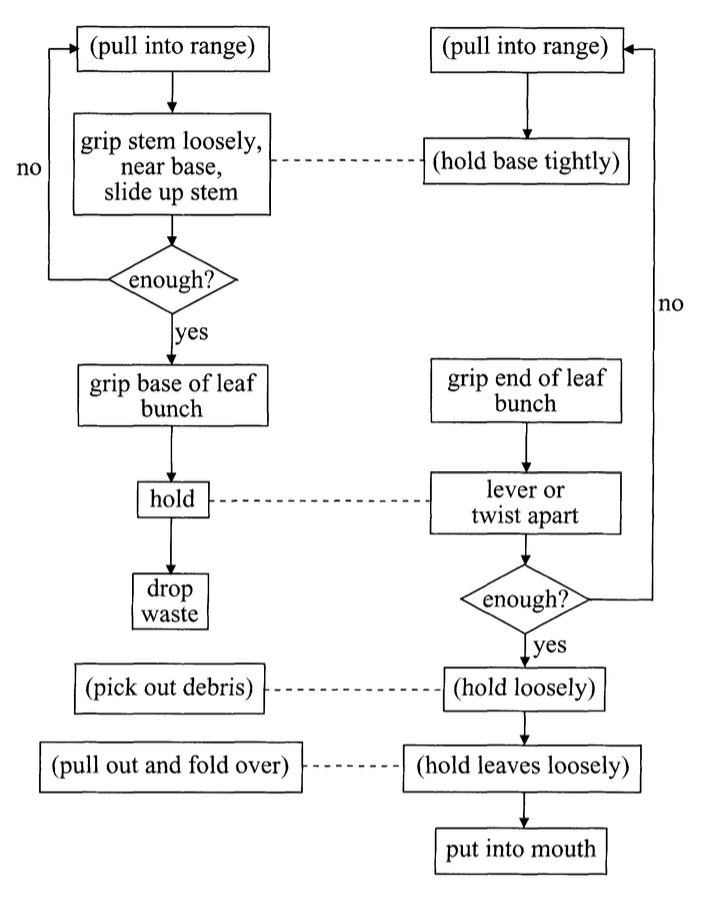
\includegraphics[scale=0.3]{img/byrne_2003_fig1.png}
\end{center}
‘great apes [are] able to acquire complex and elaborate local traditions of food
acquisition, some of them involving tool use’ \citep[p~513]{Byrne:2003wx}

Our primary concern here with behaviour reading is as a potential basis for abilities to track others’ mental states without representing them.
But behaviour reading is plausibly important in other ways.
In mindreaders, behaviour reading is thought to be useful or even necessary for identifying intentions and other mental states (\citealp[p.~861]{Newtson:1977dw}; \citealp[p.~708]{Baldwin:2001rn}).
Behaviour reading may also matter for efficiently representing events \citep{Kurby:2008bk}, identifing the likely effects of actions \citep{Byrne:1999jk}, predicting when an event likely to be of interest will occur \citep[p.~121]{Swallow:2008cf},
and learning through observation how to do things \citep{Byrne:2003wx}.
And of course a special case of pure behaviour reading, ‘speech perception’, underpins communication by language in humans.

The \emph{Birdsong Limit}: structures not found in birdsong cannot be extracted in pure behaviour reading.

‘The current study tested the hypothesis that a non-human primate species could detect abstract,
non-adjacent dependencies in acoustic stimuli, even when dependencies occurred over an arbitrary
variable number of intervening sounds ... Squirrel monkeys consistently recognized and generalized
the pattern ABnA at different levels, showing sensitivity to arbitrary-distance dependencies’
(\citealp{ravignani:2013_action}; see also\citealp{sonnweber:2015_non}).






%--- end paste
%---------------

\footnotesize
\bibliography{$HOME/endnote/phd_biblio}

\end{multicols*}

\end{document}
